\section{Intersection graphs}
\subsection{Interval graphs}

\begin{frame}{Interval graphs}

\begin{columns}
  \begin{column}{0.5\textwidth}
    \begin{figure}
    \centering
    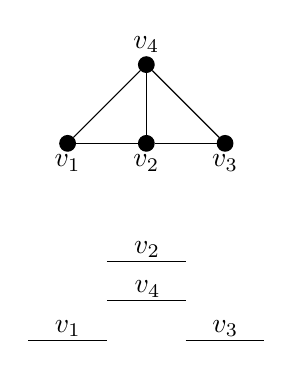
\begin{tikzpicture}

      \draw[{[-]}] (-1,-0.5) -- (0,-0.5);
      \draw[color=black] (-0.4845,-0.8507) node {$v_4$};
      \draw[{[-]}] (0,-1.5) -- (1,-1.5);
      \draw[color=black] (0.5023,-1.3568) node {$v_3$};
      \draw[{[-]}] (-2,-1.5) -- (-1,-1.5);
      \draw[color=black] (-0.4899,-0.3468) node {$v_2$};
      \draw[{[-]}] (-1,-1) -- (0,-1);
      \draw[color=black] (-1.4962,-1.3536) node {$v_1$};

      \node[draw,circle,inner sep=2pt,fill,label distance=1cm] (v1) at (-0.5,2) {};
      \draw[color=black] (-0.5,2.25) node {$v_4$};
      \node[draw,circle,inner sep=2pt,fill,label distance=1cm] (v3) at (-0.5,1) {};
      \draw[color=black] (-0.5,0.75) node {$v_2$};
      \node[draw,circle,inner sep=2pt,fill,label distance=1cm] (v2) at (-1.5,1) {};
      \draw[color=black] (0.5,0.75) node {$v_3$};
      \node[draw,circle,inner sep=2pt,fill,label distance=1cm] (v4) at (0.5,1) {};
      \draw[color=black] (-1.5,0.75) node {$v_1$};
      \draw  (v1) edge (v2);
      \draw  (v1) edge (v3);
      \draw  (v1) edge (v4);

	    \draw  (v3) edge (v2);
	    \draw  (v4) edge (v3);

    \end{tikzpicture}
    \caption{A unit interval graph with a realization.}
    \label{fig:uig_graph}
    \end{figure}
  \end{column}
  \pause
  \begin{column}{0.5\textwidth}  %%<--- here
    \begin{figure}
    \centering
    \begin{tikzpicture}

      \draw[{(-)}] (-1,-0.5) -- (0,-0.5);
      \draw[color=black] (-0.4845,-0.8507) node {$v_4$};
      \draw[{[-}] (0,-1.5) -- (1,-1.5);
      \draw[color=black] (0.5023,-1.3568) node {$v_3$};
      \draw[{-]}] (-2,-1.5) -- (-1,-1.5);
      \draw[color=black] (-0.4899,-0.3468) node {$v_2$};
      \draw[{[-]}] (-1,-1) -- (0,-1);
      \draw[color=black] (-1.4962,-1.3536) node {$v_1$};

      \node[draw,circle,inner sep=2pt,fill,label distance=1cm] (v1) at (-0.5,2) {};
      \draw[color=black] (-0.5,2.25) node {$v_4$};
      \node[draw,circle,inner sep=2pt,fill,label distance=1cm] (v3) at (-0.5,1) {};
      \draw[color=black] (-0.5,0.75) node {$v_2$};
      \node[draw,circle,inner sep=2pt,fill,label distance=1cm] (v2) at (-1.5,1) {};
      \draw[color=black] (0.5,0.75) node {$v_3$};
      \node[draw,circle,inner sep=2pt,fill,label distance=1cm] (v4) at (0.5,1) {};
      \draw[color=black] (-1.5,0.75) node {$v_1$};
      \draw  (v1) edge (v2);
      \draw  (v1) edge (v3);
      \draw  (v1) edge (v4);

    \end{tikzpicture}
    \caption{Representation of $K_{1,3}$ as a MUIG.}
    \label{fig:muigK13}
    \end{figure}
  \end{column}
\end{columns}

\end{frame}
